%%%%%%%%%%%%%%
%%% DESIGN %%%
%%%%%%%%%%%%%%

\chapter{Design}
\label{design}

This chapter presents the design process that was conducted to build a composite device that integrates smartphones to tabletops and provide a spontaneous user interaction.

A user-centered design approach was followed, in the purpose of understanding the system's context of use, and identifying the interaction techniques that would make for an intuitive application.
This process was supported by methodological tools described in Designing Interactive Systems \citep{Benyon:2010}.
Brainstorming, scenarios, storyboards and low-fidelity prototypes were used, and a study involving end users was carried out, the results of which informed the final design.

The process was focused on producing a \emph{consistent} design.
This concept was used in an effort to build an intuitive system, i.e.\ a system that users can understand without the need for conscious reasoning.
Consistency can apply to various aspects of a system design.
In the present case, the following were found to be the most relevant.
The design should aim at being consistent with (1) the user's general background, (2) the physicality of the devices and (3) the existing user experience.
The user's general background is a broad notion, that includes for example the common computer knowledge that can be expected of a user depending on his/her culture, gender, age, social background, etc.
The physicality of the devices is an important notion when designing for devices such as tabletops, because their form has decisive implications on the user's expectations.
The existing user experience refers to the user interaction that takes place on the single devices that form the composite device. Concretely, the interaction might be facilitated by keeping the experience on the tabletop consistent with the experience on the smartphone.

Due to time constraints, it was decided to limit the focus of this work to one interaction metaphor: \emph{UI replication}.
This metaphor was chosen among the possibilities enumerated in Chapter~\ref{relatedwork}, for the following reasons.
First, UI replication allows for a strong consistency between the experience on the smartphone and the one on the tabletop.
Second, UI replication can be implemented in a straightforward way, with stable protocols such as VNC \citep{Richardson:1998:vnc}, which allows the implementation effort to be focused on the interaction techniques.
Third, due to the availability of stable protocols for UI replication, the implementation can be made to support different types of smartphones.

Thus, the system is designed so as to present the user with a mirrored image of the smartphone UI on the tabletop.
This is referred to as the \emph{replicated UI}.
It is interactive, relaying touch input and graphical output between smartphone and tabletop.
The replicated UI is controlled by the \emph{surface UI}.
The surface UI consists of elements that allow the manipulation of the replicated UI on the tabletop.
\\
\linebreak
An analysis of the context of use is presented in section~\ref{sec:context}, from which solution requirements are derived in section~\ref{sec:requirements}.
Section~\ref{sec:interaction} describes the generation of design options for the surface UI and their evaluation.
The final design of the TIDE prototype is presented in section~\ref{sec:design}.

\section{Understanding the application context}
\label{sec:context}

The initial design constraints are provided by the parameters that are already known.
First, the system integrates smartphones to tabletops.
Second, the system uses UI replication to extend the smartphone UI to the tabletop.
Figure \ref{fig:useCase} describes the primary use case.
In this section, additional design constraints are derived from an analysis of the devices, and the context of use is investigated through the use of scenarios.

\begin{figure}[htb]
  \centering
    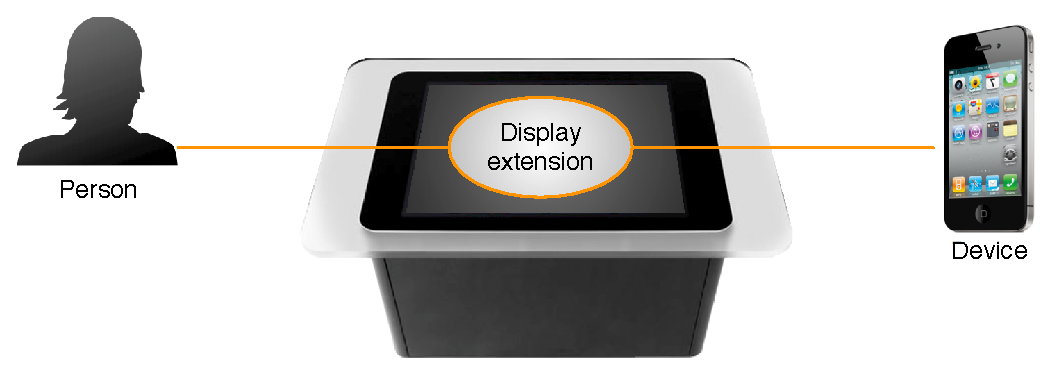
\includegraphics[width=0.9\textwidth]{images/useCase}
    \caption{Main use case.}
    \label{fig:useCase}
\end{figure}

%Most users own a computing device with personal data and applications that are tailored to their needs.
%Those personal devices are becoming smaller and more mobile, with devices such as tablet and handheld computers.
%In many cases, the display size of the personal device is a limitation in terms of graphical input and output, and has a negative influence on the user experience.
%One of the main characteristics of tabletops, however, is that they have superior graphical I/O capabilities.
%This project focuses on situations where a tabletop can be used as a display extension to the personal device, thus enhancing the user experience.

\subsection{The devices}

The basic characteristics of the devices have concrete implications on the system design.

\subsubsection{A tabletop is\ldots}

\begin{description}

\item[\ldots a computer.]
The tabletop provides computing resources such as processing power, memory and connectivity; as well as an operating system that supports software applications.

\item[\ldots a table.] 
Its physical form comprises a horizontal surface that is commonly used to support various material objects.
A table is used for various activities, such as studying, eating, playing games, holding meetings, etc.
It can be approached from all angles, encouraging face-to-face interaction between multiple users.
%The system should therefore support simultaneous users, and handle limited space availability.

\item[\ldots a situated device.] 
It usually sits at a location, and is not moved often.
It can be expected to have dedicated power supply and network connection.
Users approach it to use it, and leave when they are finished.
Thus, the interaction flow is likely to be interrupted, taking the form of short successive sessions.
The nature of the location has an impact on the user interaction, and should be considered.
Examples are a conference room, a public lobby, a mall, an individual office, a living room in a family house.
%The main implication is that tabletops seem to naturally fit in public spaces, where they are shared among multiple users.
%This tendency is accentuated by the price factor, that makes a private person not likely to buy such a device for private use.
%The system should handle public use, characterized by short anonymous sessions and an often interrupted interaction flow.

\item[\ldots a shared device.] 
When located in a public space, the tabletop is shared among multiple users.
Depending on the context, the relationship between the users varies (friends, colleagues, strangers, etc), and with it the level of trust.

\item[\ldots an interactive surface.] 
It typically offers a large graphical output, and a range of input techniques that allow user interaction.
Most tabletops support multitouch-based input.
%This introduces a new kind of interaction model, more intuitive, that the system should be based upon.
Some tabletop models support computer-vision techniques that allow the integration of tangible objects to the interaction.
%This project reports on the possibilities to use a personal device as a tangible control integrated to the tabletop.

\end{description}

\subsubsection{A smartphone is\ldots}

\begin{description}

\item[\ldots a computer.] 
It provides the computing resources necessary to allow a user to store personal data and install/use applications, as well as connectivity.
It runs on a mobile operating system that supports software applications.
%The system should allow the user to access his/her applications and personal data.

\item[\ldots a small device.] 
It is designed to fit in a pocket.
Smartphones are typically less than 5'' high, 3'' wide, and 0,6'' deep.
The small form factor implies some hardware limitations: resources such as battery life and processing power can not be taken for granted.
%However, the small form factor implies a suboptimal graphical user experience.
%The system should try to improve this, by offering superior IO resources.

\item[\ldots a mobile device.]
It is carried around by users at all times.
It is mostly used as a wireless device, across networks, implying a level of instability in the connectivity.
%The system should be developed with those concerns in mind.

\item[\ldots an interactive device.]
Modern smartphones typically include touch-based screens, as well as physical buttons, to allow user interaction.
%making them naturally suitable for display extension on a tabletop.
%The physical buttons implement strategic functions that the system should support.

\end{description}

\subsection{The situations}
\label{sec:scenarios}

Understanding the situations in which the system will be used is a step towards the elicitation of solution requirements.
The scenarios that were used to help define those situations are included in appendix \ref{scenarios}.

There are four general cases, depending on the location (public/private) and the users (single/multiple).
However, it is unclear if a location can be private when multiple users are present.
Without taking into account the nature of the relationship between the users, this configuration is an impossibility, and thus not addressed in this analysis.

\subsubsection{Single user on a public tabletop}

This situation was derived from a scenario involving a user sitting alone at an interactive table in a coffee shop.

In this environment, the motivation for using the system is an activity that involves graphically intense content, such as 
internet browsing, reading, consulting a map.
To start using the system, the user pairs the smartphone with the tabletop.
The process is quick and easy, but not completely automatic.
The user must explicitly allow the connection to be established.
The user does not usually need cables to use the smartphone.
Ideally, the connection with the tabletop is handled wirelessly.
The replicated UI appears on the tabletop, and the user starts interacting with the application.
The surface UI provides the user with features to manipulate the replicated UI, in particular: dragging, rotating and resizing.
Via the surface UI, the user can minimize and hide the replicated UI, as well as exit the application.

The smartphone itself is involved in the interaction.
Placing it on the table triggers the pairing process.
During the interaction, the replicated UI is collocated with the device, and moves together with it.
Lifting the smartphone off the table closes the connection.

%It should be possible for the user to wirelessly pair his/her personal device with a public tabletop computer.
%This implies that the devices are both connected to the local wireless networks, that they are able to detect each other and discover each other's identity on the network.
%It would not be safe to establish this connection automatically in a public space.
%Therefore, dialogs should be used both on the mobile device and on the tabletop to gather user input.
%The UI of the mobile device should be transferred to the interactive surface as graphical output, and this transferred display should be able to accept touch input to be forwarded back to the device.
%The transferred display should be contained in an application window, and this window should be manipulable (drag, resize, rotate, minimize, hide, ..).

%The application window should react to the state of the interactive surface.
%An example of this is that the application window should turn inactive if it is obstructed by an object on the table.

%\begin{itemize}
%\item{the mobile device is automatically detected by the tabletop}
%\item{dialog windows are displayed on both devices}
%\item{the wireless connection is automatic}
%\item{the mobile device UI is transferred to the surface.}
%\item{the transferred UI can be resized, rotated and moved on the surface}
%\item{the transferred UI goes inactive when objects obstruct it}
%\item{user input is forwarded to the mobile device}
%\item{the transferred UI can be minimized and restored}
%\item{the application can be exited by lifting the mobile device off the table.}
%\end{itemize}

\subsubsection{Multiple users on a public tabletop}

This situation was derived from a scenario involving some work colleagues having a meeting in a conference room equipped with an interactive tabletop.
It can be argumented that such an environment is only partly public, being only accessible to the company's employee.
However, in an effort to produce a design as generic as possible, and for the sake of simplicity, the tabletop is considered as a public device.

The motivation to use the system in this context is to view, comment and possibly edit digital data in a collaborative meeting.

Multiple users might want to connect their smartphones to the system simultaneously.
%This implies that the implementation should support parallel connections and simultaneous use.
Due to the lack of space on the table, the users remove their devices, but keep the replicated UI active on the tabletop.

%Mobile computing devices come in many forms, and ideally the system should support all of them.
%Devices vary in terms of software and hardware specifications.
%Some parameters that are especially important here are the programming platform, as well as the display resolution.

\subsubsection{Single user on a private tabletop}

This situation was derived from a scenario involving a user whose office desk is a tabletop.

The motivation for using the system is that it is a tool that the user interacts with daily, to support various activities related to the daily routine.

The tabletop being private, it can be configured so as to provide extended functionalities.
Examples of extended functionalities are: the pairing procedure can be made automatic, data can be shared between the devices.

%Some suggested functionalities are:
%\begin{itemize}
%\item automatic launch of the display extension application
%\item push application widgets from the extended display to the tabletop
%\item share data between the personal device and the tabletop
%\end{itemize}

\section{Solution requirements}
\label{sec:requirements}

There are four aspects to the system, that each relate to a specific challenge within device composition.
For each of those aspects, requirements were derived from the analysis of the application context.
Some requirements were left out, that were considered out of scope for the present work.
The requirements that were deemed essential to solving the thesis problem are formulated in this section.

\subsection{Pairing}

The pairing procedure is responsible for device discovery and connection.
It should fulfill the following requirements:

\begin{enumerate}
\item Pairing the devices should be easy and quick.
\item Discovery between the devices should be automatic.
\item Establishing the connection should require explicit confirmation from the user.
\item Automatic pairing should be an available option in trusted setups.
\item Exiting the application should be easy and quick.
\end{enumerate}

%Connecting a personal device to a tabletop should be a quick and easy process.
%The system should include a detection mechanism that would allow the devices to become aware of each other, as well as a discovery protocol to gather the information necessary to the pairing, such as a Network IP.
%The connection should be wireless to guarantee a smooth experience.
%However, a public tabletop should not be allowed to gather data from, let alone connect to, a personal device without the explicit consent of its owner.
%In the case of a trusted setup, it should be possible to bypass any explicit user input.
%Exiting the application and closing the connection should also be easy, allowing the system to handle short successive sessions.

\subsection{Replicated UI}

The replicated UI is the interactive mirror image of the smartphone displayed on the tabletop.
It should fulfill the following requirements:

\begin{enumerate}
\item The UI of the smartphone should be replicated on the tabletop.
\item The graphical output from the smartphone should be dynamically relayed to the replicated UI.
\item The touch-based input from the replicated UI should be dynamically relayed to the smartphone.
\item The responsiveness of the replicated UI should be under 1 second, to provide a satisfying user interaction.
\end{enumerate}

%At the core of the system is the display extension.
%The UI of the personal device should be transferred to the tabletop, allowing the user to interact with it in a natural way.
%Graphical output from the personal device should be forwarded to the tabletop, and touch-based input from the tabletop should be forwarded to the personal device.

\subsection{Surface UI}

The surface UI is the interface on the tabletop that controls the replicated UI.
It should fulfill the following requirements:

\begin{enumerate}
\item The surface UI should be easy to use.
\item The surface UI should allow the user to manipulate the replicated UI, i.e.\ the user should be able to move, rotate and resize the replicated UI across the tabletop display.
\item The surface UI should allow the user to minimize and restore the replicated UI.
\item The surface UI should allow the user to hide the replicated UI.
\item The surface UI should allow the user to exit the application.
\item The surface UI should include controls that implement the functionalities provided by the physical buttons present on the smartphone.
\end{enumerate}


%The user experience should be improved by using the display extension on the surface.
%Therefore, it is important to provide for a rich interaction.
%The transferred UI should be contained within a manipulable window on the tabletop.
%Specifically, the user should be able to move, rotate and resize the window; as well as minimize, hide and restore it.
%The system should include UI elements that implement the functions supported by the physical controls present on the personal device.
%Those elements and their function should be obvious to the user.
%
%%secondary features
%Modern smartphones include sensors that allow to switch the display orientation by tilting the device.
%This feature is strategic to certain applications, and should be implemented by the system.
%Obviously, tilting the tabletop is unfeasible, so another solution is necessary.
%
%As mentioned earlier, a tabletop's screen space would typically be shared among different applications and/or objects.
%Therefore, the system should handle limited screen space, and obstruction of the display extension.
%
%In a trusted setting, the user should have the possibility to push application widgets from the personal device to the tabletop, outside of the display extension, thus saving space on the latter.

\subsection{Tangible UI}

The tangible UI is the set of features that are used by physically interacting with the smartphone.
It should fulfill the following requirements:

\begin{enumerate}
\item Placing the smartphone on the tabletop should trigger the pairing procedure.
\item The replicated UI should be collocated with the smartphone, i.e.\ the replicated UI should be seemingly linked to the device, and should move when the device is moved.
\item Lifting the smartphone off the table should trigger the application exit.
\item It should be possible to remove the smartphone, but keep the replicated UI active the tabletop.
\end{enumerate}

%It is a natural thing to place an object on a table, and tabletops are designed to allow for the integration of physical artifacts.
%Therefore, it should be possible to use the personal device as a tangible UI.
%For example, it would seem obvious that placing the device on the tabletop would launch the pairing process, or that lifting it off would interrupt the connection.
%Furthermore, it should be possible to control the position of the display extension by sliding the personal device on the surface.

\section{Designing the user interaction}
\label{sec:interaction}

This section focuses on the design of the surface UI, which comprises the UI elements that provide control over the replicated UI on the tabletop.

It was decided to focus exclusively on touch-based interaction in the design of the surface UI, for the following reasons.
First, it is consistent with the physicality of tabletops, who rely on touch-based input to provide an appealing experience to all types of users.
Second, it is consistent with the smartphone experience, which also relies on touch-based input.
Lastly, the presence of other input peripherals cannot be expected, so relying on touch-based input will ensure that the system is compatible with any setup.

The steps followed to design the surface UI were: (1) the generation of ideas, (2) the definition of \emph{interaction strategies }and (3) a study involving end-users to identify the most intuitive interaction techniques.

%The pairing procedure does not introduce anything new to the field. There are known solutions to this challenge, which are described in section \ref{}.
%The remote UI replicates the UI of the personal device on the tabletop, and does not require any supplementary design.
%Using the personal device as a tangible UI for the display extension raises a series of design and implementation challenges. It is the opinion of the author that this research angle is promising, but it was decided to leave it out of the project for reasons of time constraints.
%\hfill\\

\subsection{Generating ideas}

The generation of ideas is an important part of the design process.
Benyon refers to it as envisionment \citep{Benyon:2010}, which he defines as the process of externalizing design thoughts.
The techniques that were used to permit this process are brainstorming, sketching, storyboarding and prototyping.

\subsubsection{Storyboards}

The scenarios mentioned in section~\ref{sec:scenarios} are used as a base for the making of storyboards.
Storyboarding helps getting a feeling for the general flow of the interaction with the system.
It also gives a visual dimension to the definition of the different system features, and raises new design issues.
Putting orally expressed ideas on the paper is often a first test of their validity.

For example, several system features were described in the initial scenarios as being the effect of a tap on a button.
When storyboarding, it became obvious that having too many UI buttons would be cumbersome, which lead to the consideration of other interaction techniques, such as touch gestures.
Similarly, the issue of the location and size of the replicated UI on application launch became first apparent on a storyboard.

\subsubsection{Low fidelity prototypes}

Paper prototypes were used to aid the process of generating and evaluating as many design solutions as possible.
Screenshots of the iPhone UI \citep{iphone} were printed out in various sizes, and used on a normal table to simulate interaction with the replicated UI.
Figure \ref{paperProt} shows some prototypes and a working session.

\begin{figure}[htb]
  \centering
    \includegraphics[width=1\textwidth]{images/paperProtDouble}
  \caption{Working with low fidelity prototypes.}
  \label{paperProt}
\end{figure}

%\begin{figure}[h!]
%  \caption{Low fidelity prototypes.}
%  \centering
%    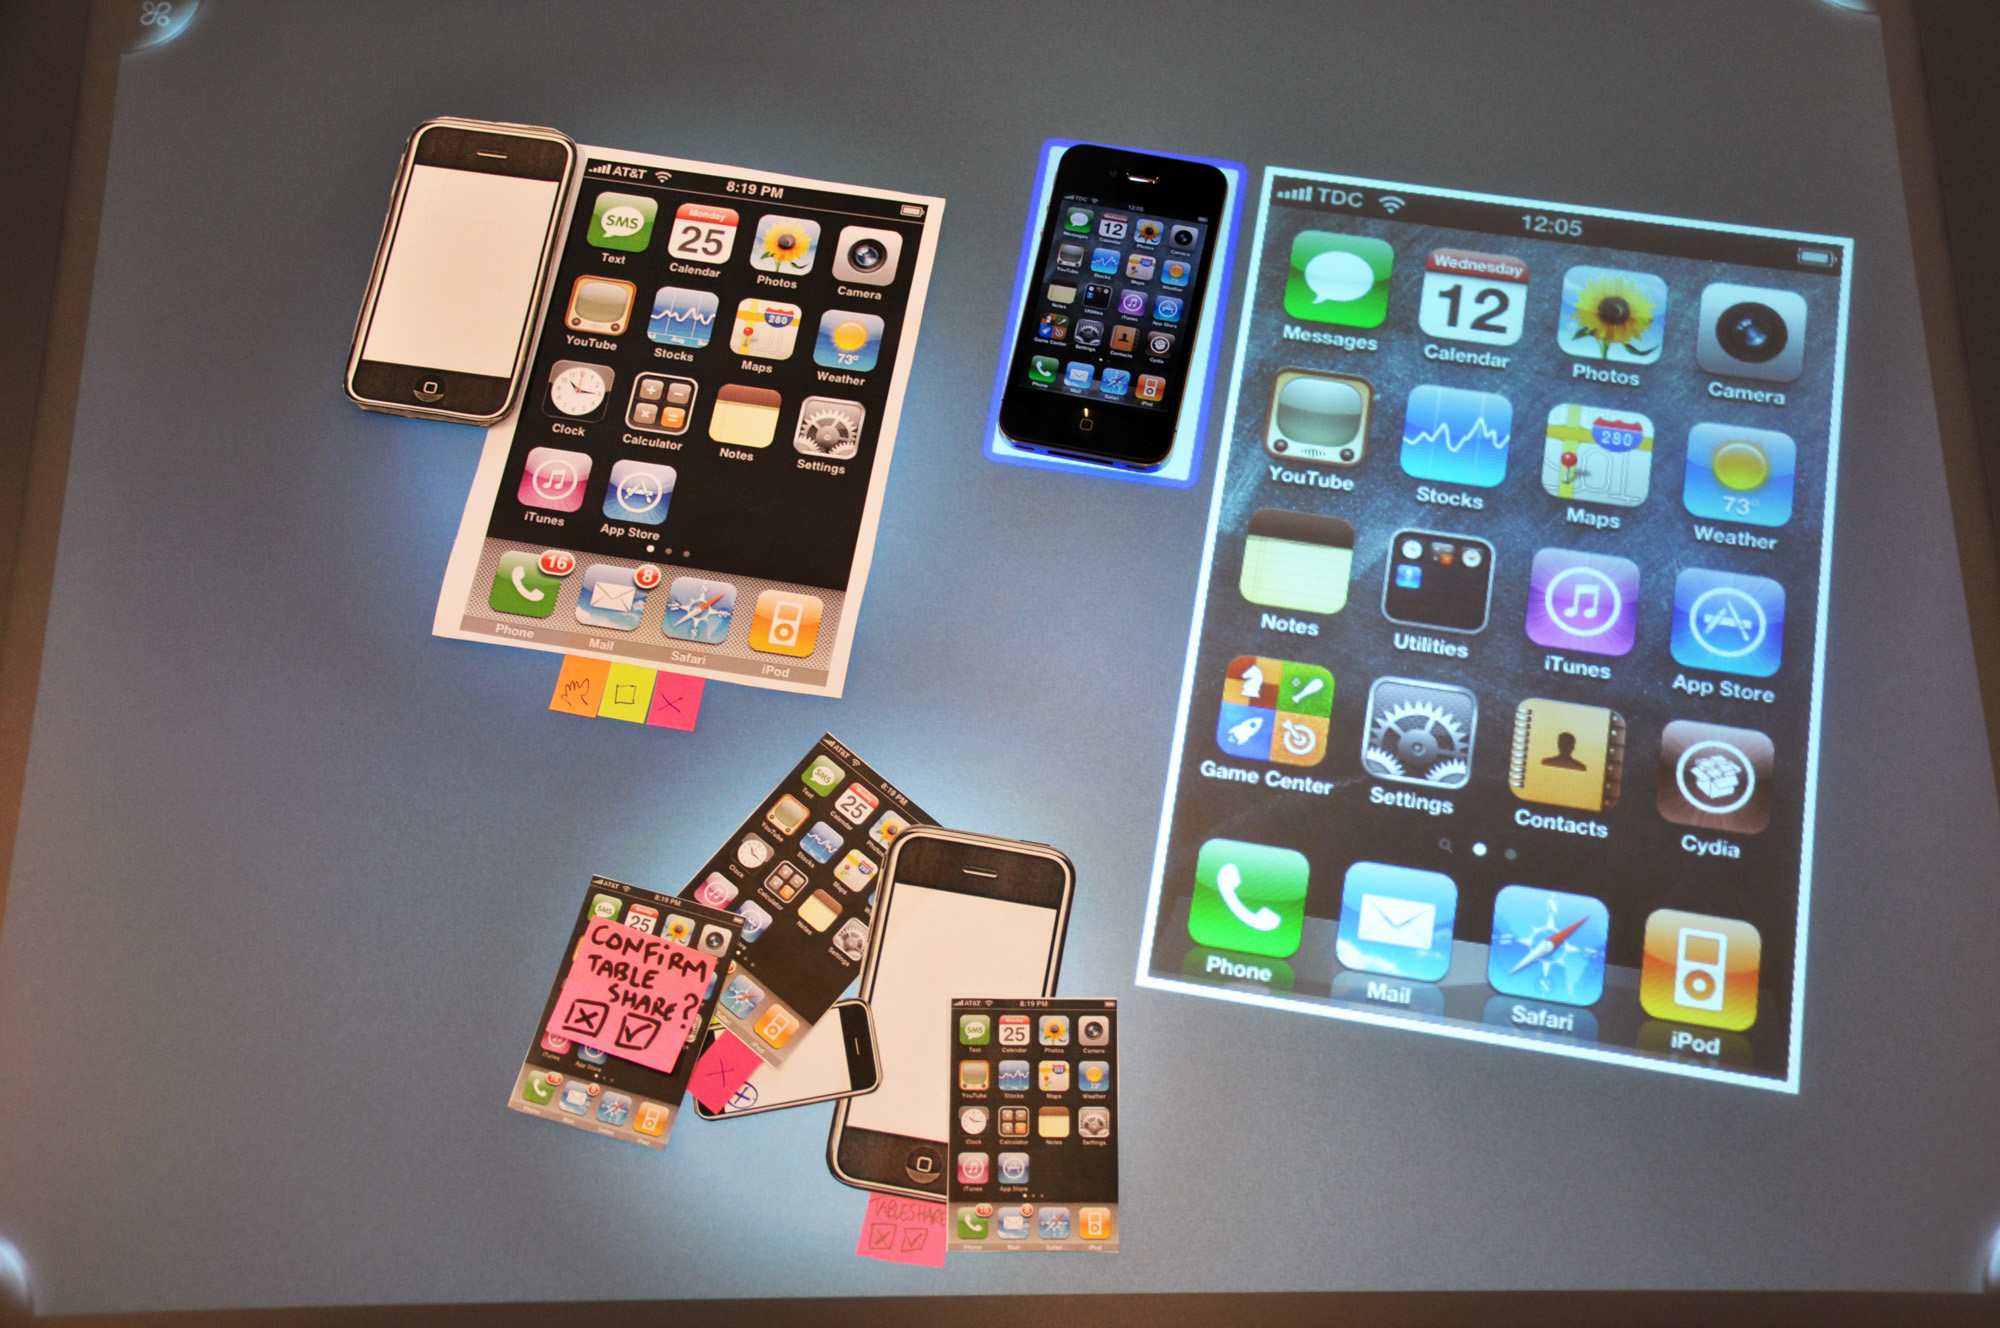
\includegraphics[width=0.8\textwidth]{images/paperprot2}
%\end{figure}

%\begin{figure}[h!]
%  \caption{Low fidelity prototypes.}
%  \centering
%    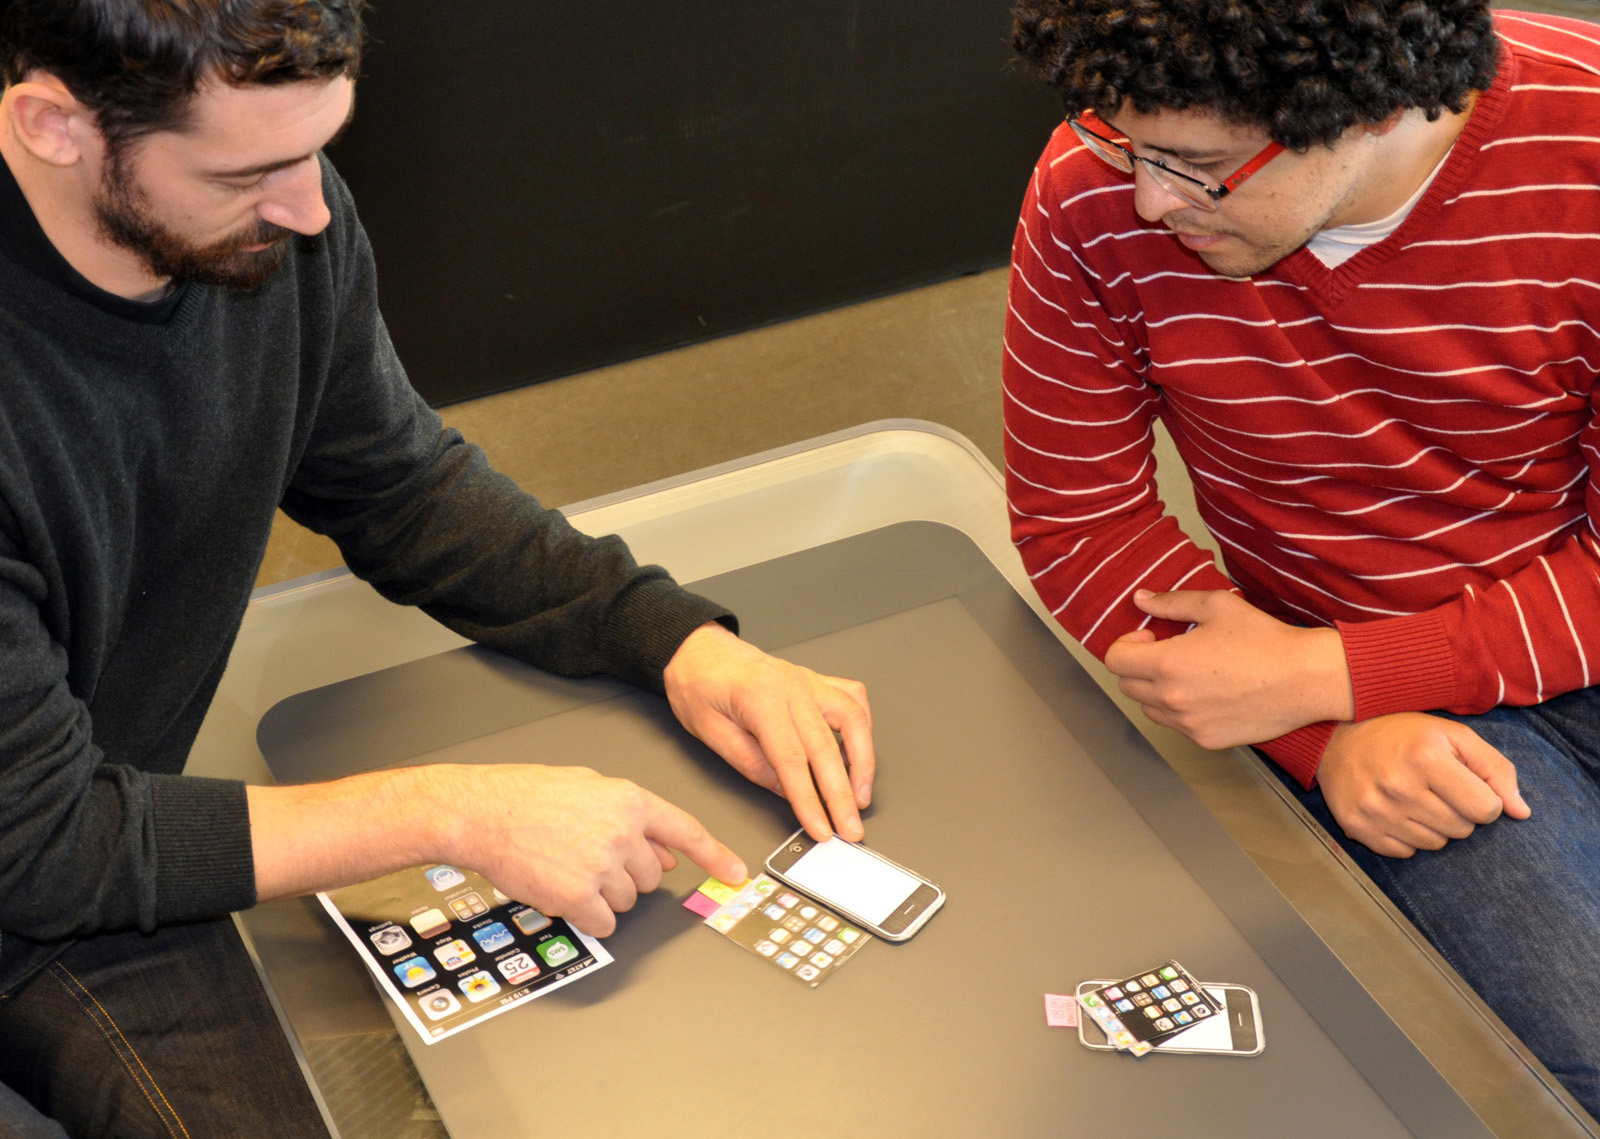
\includegraphics[width=0.8\textwidth]{images/paperprot3}
%\end{figure}

\subsection{Defining interaction strategies}
\label{sec:strategies}

The concepts of \emph{actions} and \emph{commands} are used to refer to the different interaction strategies.
They are inspired by the work done by Wobbrock et al. on defining hand gestures for interactive surfaces, \citep{Wobbrock:2009:gestures}.

Human computer interaction can be modeled as a simple cause-effect relationship.
The user wishes the computer to execute a command.
To achieve that, s/he performs an action to provide input.
In the case of a touch-based interactive surface, the action is typically a hand gesture.
The action is the cause, the command is the effect, and together they form a single interaction between user and machine.

\subsubsection{Commands}

The following six basic commands are identified as interaction primitives for the surface UI.
They are directly derived from the requirements formulated in section~\ref{sec:requirements}.

\begin{enumerate}
\item{\emph{Dragging} the replicated UI across the interactive surface.}
\item{\emph{Rotating} the replicated UI across the interactive surface.}
\item{\emph{Resizing} the replicated UI across the interactive surface.}
\item{\emph{Minimizing} the replicated UI, and restoring it.}
\item{\emph{Hiding} the content of the replicated UI.}
\item{\emph{Exiting} the application.}
\end{enumerate}

Additionally, the surface UI should include controls that implement the functionalities provided by the physical buttons present on the smartphone.

\subsubsection{Actions}

Various interaction techniques can be used to invoke application level commands.
% as shown in figures~\ref{fig:strat1} to \ref{fig:strat4}.
While working with paper prototypes to generate ideas, it became apparent that some interaction techniques could be regrouped into categories that could be consistently implemented for each of the previously defined commands.
This realization lead to the definition of five interaction strategies.
There is a sixth category, that regroups design suggestions that are not part of any consistent strategy.

\begin{enumerate}
\item{\emph{Action Tabs} are traditional buttons/tabs that implement functionalities (figure~\ref{fig:strat1}).}
\item{The \emph{Action Bar} can be compared to a virtual touchpad, it includes a manipulation area and buttons (figure~\ref{fig:strat2}).}
\item{\emph{Window Toggle} refers to using a switch to toggle the window between inactive and active states. In its inactive state, the window is made manipulable as a common digital picture.}
\item{The \emph{Active Border} is a digital frame around the application window used for manipulation (figure~\ref{fig:strat3}).}
\item{\emph{Active Corners} is a strategy similar to Active Border, with the difference that the border's corners implement specific functionalities (figure~\ref{fig:strat4}).}
\item{\emph{Other} regroups suggestions that do not fit with any specific strategy.}
\end{enumerate}

\begin{figure}[ht]
\begin{minipage}[b]{0.5\linewidth}
\centering
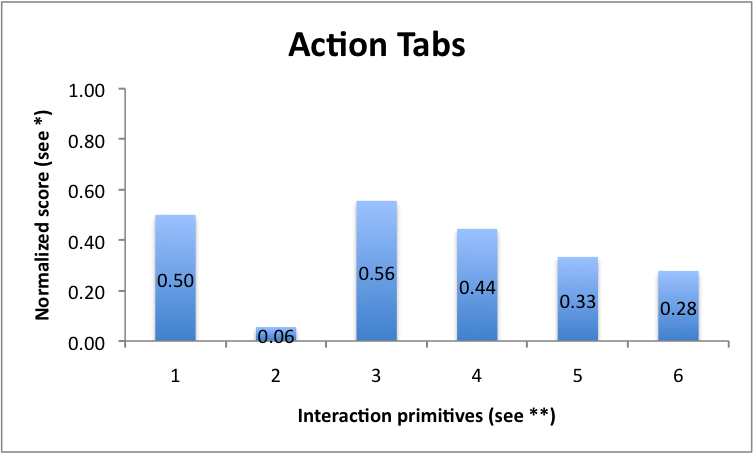
\includegraphics[width=0.6\linewidth]{images/strat1}
\caption{action tabs prototype}
\label{fig:strat1}
\end{minipage}
\hspace{0.5cm}
\begin{minipage}[b]{0.5\linewidth}
\centering
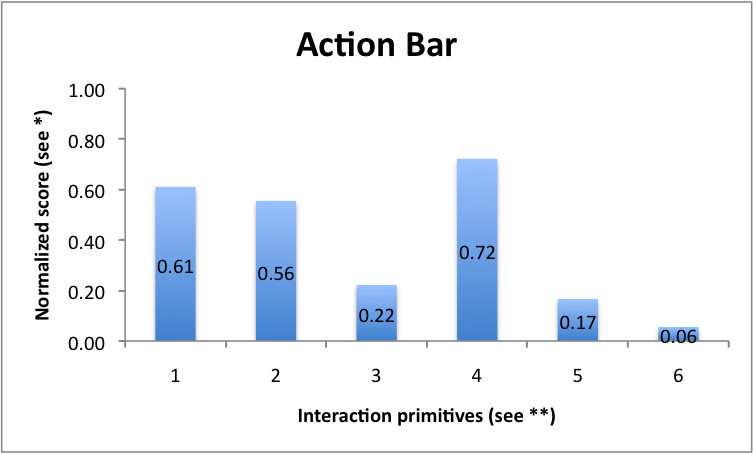
\includegraphics[width=0.6\linewidth]{images/strat2}
\caption{action bar prototype}
\label{fig:strat2}
\end{minipage}
\hfill\\
\begin{minipage}[b]{0.5\linewidth}
\centering
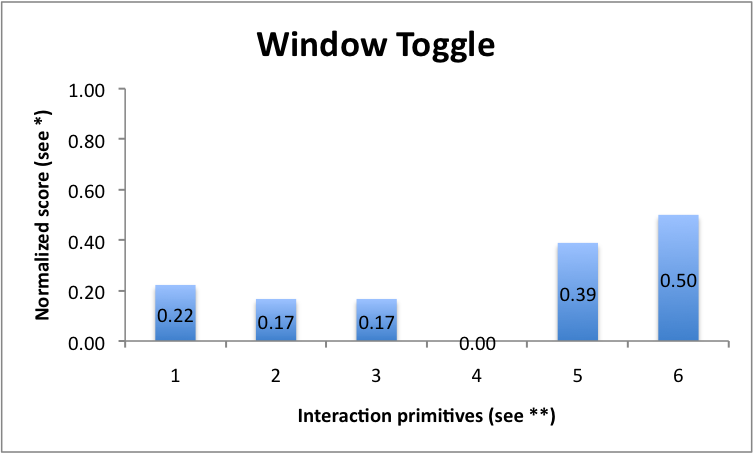
\includegraphics[width=0.6\linewidth]{images/strat3}
\caption{active border prototype}
\label{fig:strat3}
\end{minipage}
\hspace{0.5cm}
\begin{minipage}[b]{0.5\linewidth}
\centering
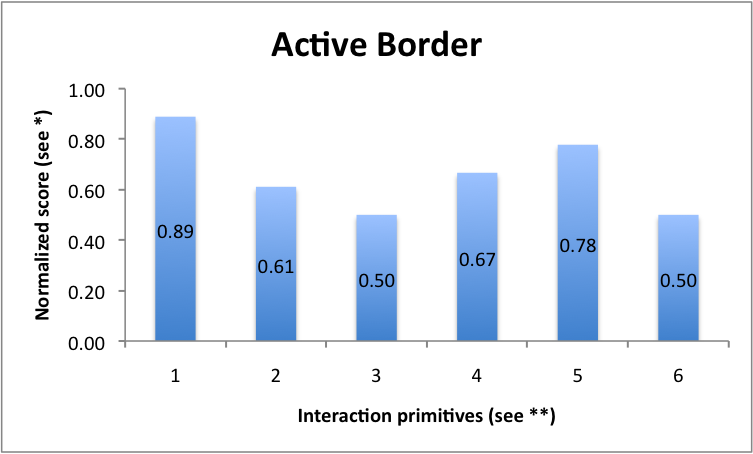
\includegraphics[width=0.6\linewidth]{images/strat4}
\caption{active corners prototype}
\label{fig:strat4}
\end{minipage}
\end{figure}

\subsection{Involving users}

To discover which of the defined interaction strategies were most intuitive, an experiment was carried out, that involved end users.
The experiment took the form of cooperative design sessions, where users engaged with low-fidelity prototypes of the system, in the aim of exploring and evaluating ideas.

The parameters of the experiment are the commands, also referred to as \emph{interaction primitives}, and the actions, also referred to as \emph{interaction strategies}, defined in section~\ref{sec:strategies}.

The interaction primitives are central system features.
For each primitive, the participants were asked to express an open-ended \emph{user suggestion}, then to \emph{rank} the interaction strategies.

\begin{figure}[htb]
  \centering
    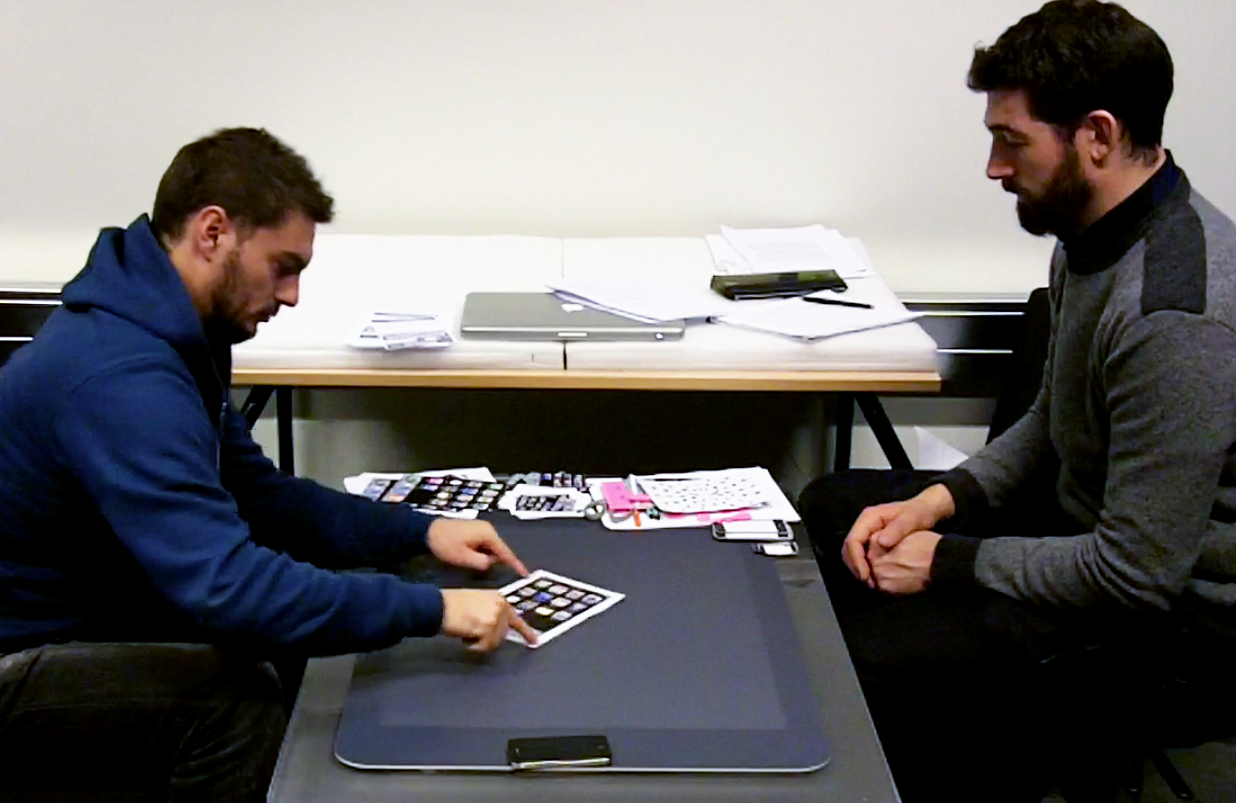
\includegraphics[width=0.8\textwidth]{images/studyScreenshot}
  \caption{Experimenting with prototypes.}
  \label{studyScreenshot}
\end{figure}

\subsubsection{Experiment}

Twelve participants were recruited on a voluntary basis.
A session involves one participant and one designer.
The participant sits next to the Microsoft Surface tabletop \citep{ms}, and is presented with an iPhone \citep{iphone}, but both devices are off.
On the tabletop are paper prototypes, that are to be used as representations of UI elements throughout the session.
The designer leads the experiment by reading instructions from a script (included in appendix~\ref{app:study}) and answering the participant's questions.
\\
\linebreak
As an introduction, the following things are explained to the participant:
\begin{itemize}
\item the purpose of the experiment,
\item the purpose of the application,
\item the tasks that the participant will perform,
\item the principles of working with paper prototypes.
\end{itemize}
\hfill
\linebreak
The session revolves around a task that the participant is asked to perform using the prototyped application.
The task is to write an email, and it requires the user to go through six phases.
Each phase is dedicated to an interaction primitive, and they have the same structure, which is as follows:
\begin{enumerate}
\item the primitive is explained to the participant in terms of a command to the application,
\item the user is asked to express an open-ended suggestion, i.e.\ suggest an action that s/he would perform to obtain the desired effect, and to demonstrate the action using the prototypes,
\item the designer describes action suggestions, that the user is asked to try out and rank by order of preference.
\end{enumerate}

%There is a seventh phase focusing on the pairing procedure.
%This phase occurs first and is meant as an example to the participant, describing the common structure.
%At the end of this phase, a slide animation is used to describe all six primitives to the user.

For each command, there are six possible actions.
However, it was decided that presenting a user with six options to rank would be overwhelming.
The volunteers were therefore split into two groups, each evaluating a subset of the interaction strategies.
The repartition is shown in table~\ref{groups}.

\begin{figure}[htb]
  \centering
    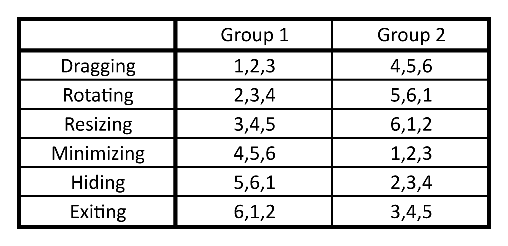
\includegraphics[scale=1]{images/groups}
  \caption{The repartition of the evaluated interaction strategies between the two groups of participants. The strategies are 1)~Action Tabs 2)~Action Bar 3)~Window Toggle 4)~Active Border 5)~Active Corners 6)~Other.}
  \label{groups}
\end{figure}

%Figure \ref{studyScreenshot} shows a typical experiment session.

\subsubsection{Data processing}

Participant answers were gathered in a form such as the one included in appendix~\ref{app:studyForm}.
The form is a matrix where an entry corresponds to a pair (primitive,strategy).
Those entries contain the position from first (highest) to third (lowest), that was given by the user for using the suggested strategy for implementing the primitive.
After processing all answers, each entry contains 6 positions.
In order to obtain a numeric score for each entry, a weighted average was calculated, giving a weight of 3 to a first position, a weight of 1 to a second position, and a weight of 0 to a third position.
Finally, the results were normalized to a [0-1] interval, where a 1 signifies that the entry was awarded a first position by all participants, and a 0 signifies that all participants ranked this entry third.
Figure~\ref{resultMatrix} summarizes the normalized scores, with colored cells containing values above 0.6.
This is considered a superior score, because it can only be obtained if half of the participants awarded the first position.
%The same results are presented in the form of charts in figure~\ref{primitives}.

The experiment data also included the user suggestions, gathered separately on paper.
User suggestions were not limited to one per primitive, so the processed data was a disparate list of suggestions that each had a counter variable indicating how many users independently expressed said suggestion.

\begin{figure}[htb]
  \centering
    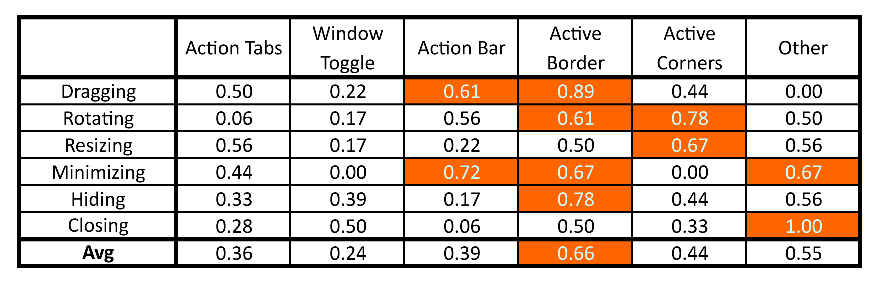
\includegraphics[scale=1]{images/resultMatrix}
  \caption{Normalized weighted average of the ranks given to each pair (primitive, strategy).}
  \label{resultMatrix}
\end{figure}

%\begin{figure}[h!]
%  \centering
%    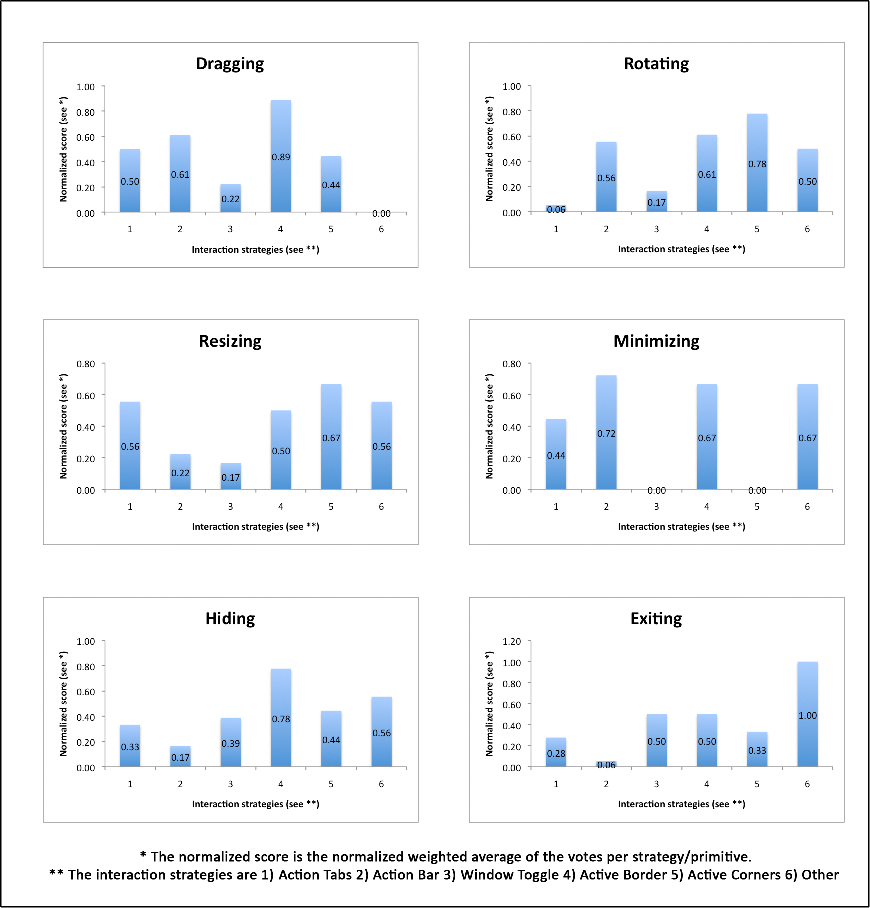
\includegraphics[width=1\textwidth]{images/primHistog}
%    \caption{The score of the different interaction strategies for each primitive.}
%	\label{primitives}    
%\end{figure}

\subsubsection{Result Analysis}

It is possible to divide the primitives into two groups.
The first half: dragging, rotating, resizing; have a concrete visual signification.
The second half: minimizing, hiding, exiting; are more abstract.

For the first three primitives, there is a strong coherence in the choice of the participants.
The favored strategies are the active border, the action bar and active corners.
All three require the user to interact with an area directly around the window in order to manipulate it and modify its position, orientation or size.
This interaction strategy is similar to the current standard for manipulating pictures on interactive screens, with the difference that in the present case, the replicated UI is logically avoided because of its role as IO relay between the tabletop and the smartphone.

For the last three primitives, the action bar and active border continue to score high, even though there is no apparent relation between the visual aspect of the strategy and the effect implied by the command.
To understand this, it is necessary to look at the actual suggestions.
The favored strategies for minimizing were double tapping on the action bar and double tapping on the active border.
For hiding, the favored strategy was double tapping on the active border.
It is thus obvious that it is the double tap that participants have a preference for, possibly because it is a common technique in many other application contexts, as well as a quick and easy one.

It is not possible to analyze the scores of the sixth interaction strategy as a whole, as it does not represent a consistent strategy, but more a patchwork of various suggestions, that were chosen because of their originality and interest. They are:
\begin{enumerate}
\item Drag by holding a finger on a specific tab, and using another finger to tap a destination target to move the window to.
\item Rotate by performing a one finger dragging gesture on a corner of the window.
\item Resize by pulling the window apart with both whole hands.
\item Minimize by dragging the window to the bottom of the surface.
\item Hide by placing and holding a full hand on the window.
\item Exit by dragging the window to a specific location on the surface.
\end{enumerate}
Suggestions 4 and 6 are similar, and they are the only ones that scored above 0.6.
This suggests that moving the window off screen is a natural way to remove focus from the application.
Interestingly, this correlates with the analysis of the user suggestions.
\\
\linebreak
The user suggestions were multiple and heterogeneous, but data processing revealed a clear tendency in three situations.

In the case of dragging, half of the participants suggested using one or more fingers to touch within the replicated UI, and perform a drag gesture.
This is interesting, because it is an obvious conflict for the developer, i.e.\ any touch inside the replicated UI is forwarded to the smartphone, and can logically not be interpreted by the surface UI.
It must be noted that dragging was the first primitive, and it can therefore be assumed that the participants did not yet have a full understanding of the application concept.
However, this result shows what the ideal system should be able to do: interpret the intention of the user.

In the case of resizing, 8 out of 12 participants suggested grabbing the sides of the window with 2 fingers, and pulling the window apart to enlarge it.
This shows that the gesture is very intuitive, and that implementing it would definitely add to the usability of the system.

The third consensus was for minimizing, where 7 out of 12 participants suggested dragging the window offscreen (or to a specific location along the surface edge).
The same suggestion reoccurred for the primitives hiding and exiting, though with less decisiveness.
Once again, it shows that the gesture is an intuitive one.
Moreover, it is consistent with the action of removing a real piece of paper from the center of a table.
%, and the act of minimizing, hiding or exiting the display extension application.
%Moving the application out of focus seems like a good solution, and using a simple dragging gesture is a natural way of doing it.

\section{Final Design}
\label{sec:design}

%This project focuses on UI replication because it improves the user experience while keeping the interaction natural, and it can be implemented with the available resources.
%On a technical level, the advantage of UI replication is that it uses the application logic of the personal device, requiring of the remote display only to forward graphical output, and touch-based input.
%This allows the development of software that is easily adaptable to various programming platforms.
%On a human-computer interaction level, it reduces the learning curve for the user, by providing an intuitive experience that is similar to the one s/he is used to.
%By comparison, the streaming metaphor is too limited, and the other paradigms all introduce new interaction dimensions that require user adaptation.
%A final argument in favor of UI replication is that it allows the implementation of an engaging prototype without requiring any additional graphical design.

The experiment provided precious input from potential users, and this input supported the initial views that in order to build a successful system, the focus should be on usability and intuition.
In this context, intuitive interaction means that the user should be able to learn the system through free exploration, all the time guessing and discovering functionalities.
To allow this phenomenon, the implementation should focus on three things.
First, it should be coherent. If the features are consistent, the user will be able to derive one from the other.
Second, common interaction techniques should be used, such as the picture manipulation gestures (drag, pinch, rotate) that are already successful on touch-based interactive screens.
Third, the implementation should refer to the table metaphor when possible, using the user's familiarity with normal table objects to hint at specific features.\\
\hfill\\
The implementation choices are as follows:
\begin{itemize}
\item Dragging, rotating and resizing are done by manipulating an active border that frames the window. The active border has the visual appearance of the body of the physical device.
\item When the window is dragged off an edge of the table, the application is minimized. Minimizing can also be done by double tapping the active border.
\item In its minimized state, the application appears as an icon on the tabletop. This icon can be moved around, restored, or closed.
\item On closing the application, the user will be prompted to confirm exiting the application.
\item Exiting can also be done by dragging the window to a corner of the tabletop, or by pressing and holding one finger on the active border.
\item Hiding is achieved by minimizing the application. Minimizing is therefore also implemented as a result of holding a whole hand over the window.
\item When reduced under a certain threshold, the application is minimized. Similarly when enlarged above a certain size, it is maximized to a fullscreen mode. To escape the fullscreen mode, buttons are implemented in the corners of the tabletop.
\item the buttons present on the physical device are a logical part of the active border, and their functions are implemented accordingly.
\end{itemize}
\hfill\\
In most software applications, there exists two ways to activate the same command.
The advantage is that one implementation can be made to be easy to discover, while the other is more obscure, but a faster or easier interaction.
The best example of this are keyboard shortcuts. They can not be guessed by the novice user, but they are used by the expert user for their efficiency.
Similarly, the display extension can be minimized easily and quickly by double tapping the active border, but the novice user can easily discover the feature by simply dragging the window off screen.
